\section{Gestione utenti}
\label{gestioneutenti}
Per accedere alla pagina di gestione degli utenti, cliccare sul link Users (1) (vedi figura \ref{fig:users}) presente sulla barra dei menù.

\begin{figure}[H]
	\centering 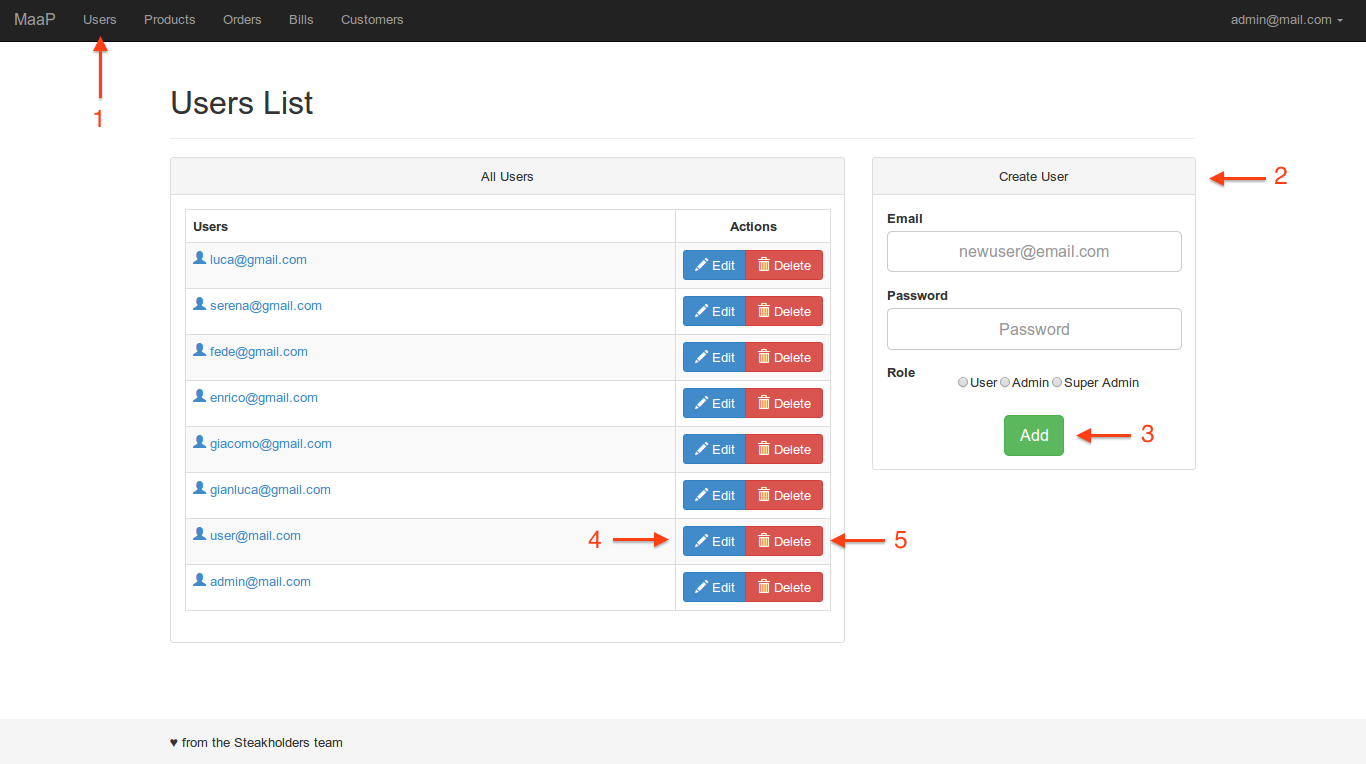
\includegraphics[width=1\textwidth]{img/users.png}
	\caption{ \label{fig:users} Pagina Users List}
\end{figure}


	\subsection{Visualizzazione}
	\label{utenti-visualizzazione}
	Per visualizzare i dettagli di un utente, cliccare sull'indirizzo mail corrispondente al suo profilo. Inoltre, è presente un pulsante \texttt{Edit User} (1) (vedi figura \ref{fig:visualizzautente}) per modificare l'utente selezionato (vedi paragrafo \ref{utenti-modifica} per la modifica dell'utente).

	\begin{figure}[H]
		\centering 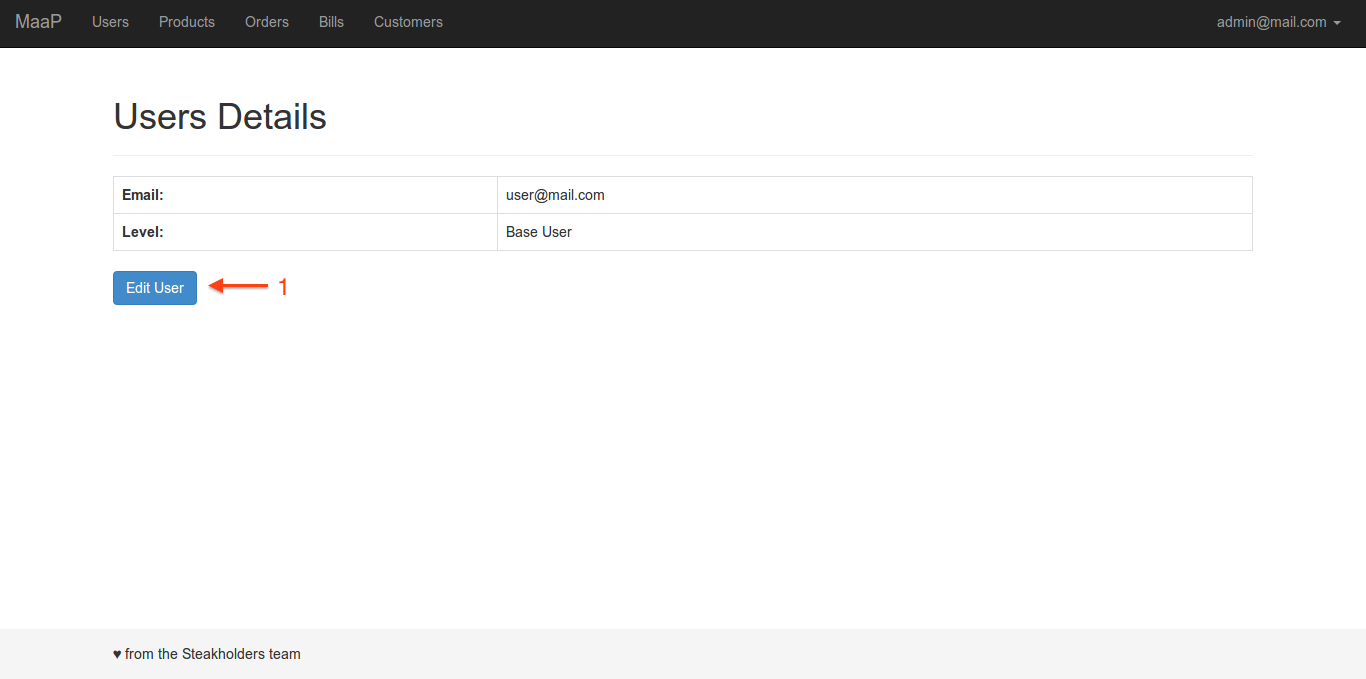
\includegraphics[width=1\textwidth]{img/visualizza-utente.png}
		\caption{ \label{fig:visualizzautente} Pagina di visualizzazione dettagli utente}
	\end{figure}

	
	\subsection{Inserimento}
	\label{utenti-inserimento}
	Per inserire un nuovo utente, compilare il form \texttt{Create User} (2) (vedi figura \ref{fig:users}) definendo email, password e livello dei privilegi. Una volta aver cliccato sul pulsante \texttt{Add} (3), se i dati inseriti sono validi, il nuovo utente verrà inserito nella lista degli utenti, altrimenti verrà visualizzato un errore.


	\subsection{Modifica}
	\label{utenti-modifica}
	Per modificare un utente, cliccare sul pulsante \texttt{Edit} (4) (vedi figura \ref{fig:users}) associato all'utente che si vuole modifica. Nella pagina visualizzata è possibile modificare il livello dell'utente tramite il form apposito.


	\subsection{Eliminazione}
	\label{utenti-eliminazione}
	Per eliminare un utente, cliccare sul pulsante \texttt{Delete} (5) (vedi figura \ref{fig:users}) associato all'utente che si vuole eliminare. Nell'\glossario{alert} che viene visualizzato è richiesta la conferma dell'eliminazione. Cliccare su \texttt{Ok} per confermare, altrimenti cliccare su \texttt{Cancel} (vedi figura \ref{fig:alerteliminazioneutente}).

	\begin{figure}[H]
		\centering 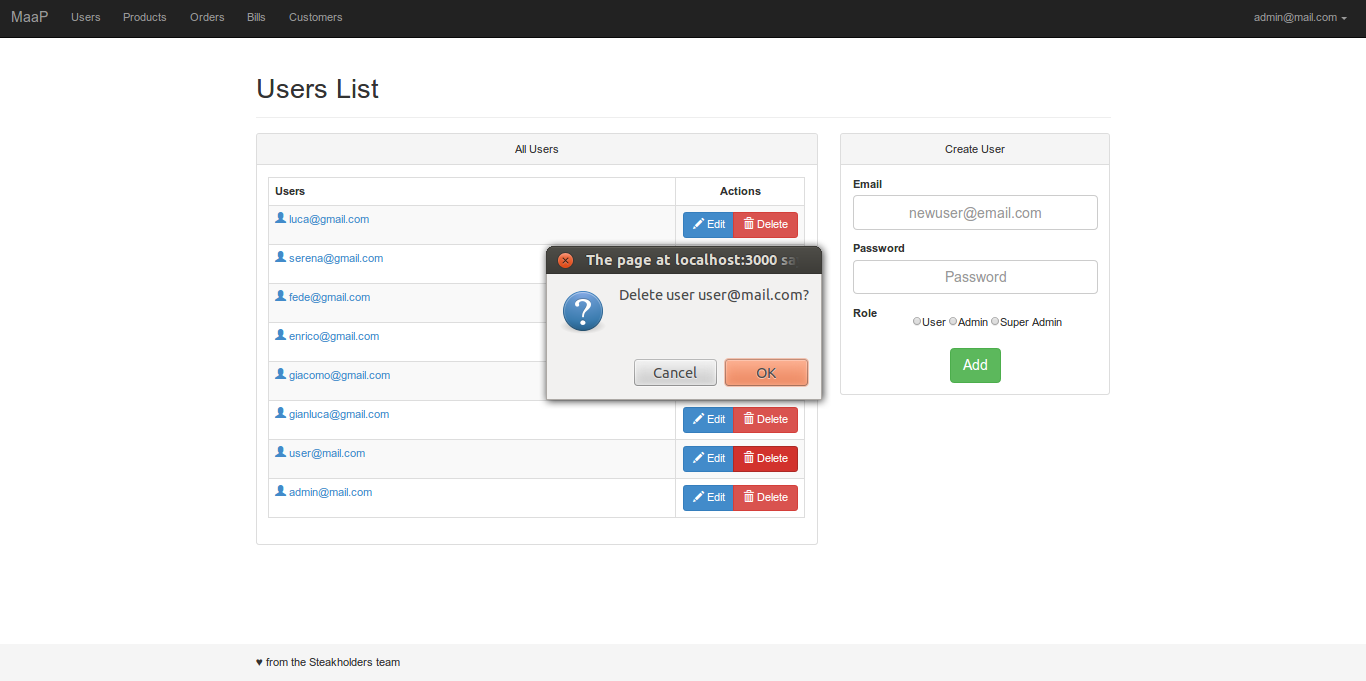
\includegraphics[width=1\textwidth]{img/alert-eliminazione-utente.png}
		\caption{ \label{fig:alerteliminazioneutente} Alert di conferma eliminazione utente}
	\end{figure}